\documentclass[a4paper, 14pt]{report}

\usepackage{cmap}
\usepackage[T2A]{fontenc}
\usepackage[utf8]{inputenc}
\usepackage[english,russian]{babel}
\usepackage[left=30mm, top=20mm, right=20mm, bottom=20mm, nohead, nofoot]{geometry}
\usepackage{indentfirst}

\usepackage{amsmath}
\usepackage{MnSymbol}
\usepackage{wasysym}

\usepackage{pgfplots}

\usepackage{graphicx}
\graphicspath{{img/}}
\DeclareGraphicsExtensions{.pdf}

\usepackage{tikz}
\usetikzlibrary{graphs}

\usepackage{multirow}

\usepackage[most]{tcolorbox}
\newtcolorbox{lbox}[2][] {
    enhanced,
    sharp corners,
    colback=white,
    colbacktitle=white,
    coltitle=black,
    boxed title style={colframe=white},
    attach boxed title to top center={yshift=-3mm},
    title=#2,#1
}

\author{Рязанова Наталья Юрьевна}
\title{Операционные системы}
\date{2019}

\begin{document}
\maketitle

\tableofcontents
\clearpage

\chapter{История}

Деления на поколения можно считать очень условными.

\textbf{Компьютер} - программно управляемое устройство.

Современным ПК часть времени управляет ОС, часть времени - приложения.

\section{Первое поколение}

В 40-х годах потребность в больших, быстрых, точных вычислениях увеличилась из-за гонки вооружений.

\begin{itemize}

    \item В 1944 году в США была создана MARK I - первая вычислительная машина на электромагнитных реле.

    \item В 1946 году - первая электронно-цифровая машина на электро магнитных лампах - UNIVAK.

    \item 1945-46 гг. - создание первого поколения ЭВМ. Длился до 1955 года. Особенности: использовались электронные лампы, ЗУ на линиях задержки, ЗУ вращающегося типа, концепция хранения программ. Для ввода/вывода - перфокарты, печатающее устройство.
\end{itemize}

Первые серийные машины - MARK I, UNIVAK I, LEO I.

Все программы выполнялись в \textbf{абсолютных адресах} - адресах байта/слова (2 байта) и т.д. физической памяти. В эти же годы разработали ENIAC. В группу разработки в 1944 г. вошел Джон Фон Нейман. В 1945 г. он опубликовал доклад, в котором определены основные принципы построения компьютерной машины, которую называют компьютером. В 1946 г. - статья "Предварительная конструкция ЭВУ", в ней была описана формальная огранизация работы машины.

\textbf{Принцип хранимой программы} - данные и команды хранятся в одной памяти. Для того, чтобы к ним отбращаться, они хранятся в опредеенных адресах. Требует это счетчик команд, он хранит адрес следующей команды.

\section{Второе поколение}

С середины 50-х годов - отсчет второго поколения ЭВМ. Появились диоды и триоды (транзисторы) и ОЗУ на магнитных сердечниках.

Для серийного производства машины нужна техническая документация.

\begin{tikzpicture}
    \graph[nodes={rectangle,draw=black}, grow right sep=1em]{
        IBM 1401 -> IBM 7094 -> 1401
    };
\end{tikzpicture}

Для автоматического перескока с 1 задания на другое понадобилось специальное ПО, которое стали называть ОС. Была создана серия оберточных и отладочных программ, которые помогали программису. Для управления заданиями был разработан специальный язык - язык управления заданиями.

\section{Третье поколение}

С начала 60-х годов - 3 поколение ЭВМ. Появились микросхемы. К 3 поколению относится полноценное появление \textbf{архитектуры ЭВМ}. Появилось в связи с идеей мультипрограммными обработками и реализацией распаралеливания фукнций. Для ускорения переключения между заданиями - загрузка нескольких заданий в ОЗУ.

Большое число программ разделяет одно адресное пространство физической памяти.

\textbf{Процесс} - программа в стадии выполнения.

Перед ОС появились новые задачи, появился менеджер памяти для выделения/распределения/очищения. Нужно было обеспечить защиту защиту памяти выделенной для программы.

В 3 поколении появилась начальная архитектура. \textbf{Канал} - программно управляемое устройство, в задачи когорого входило управление внешними устройствами.

IBM 360 - машина третьего поколения.

\hfill

\begin{tikzpicture}
    \graph[nodes={align=center,rectangle,draw=black}, grow down sep, branch right sep]
    {
        Proc -> Memory ->
        {
            "Multiplex channel" -> YVV1,
            "Spector channel" -> YVV2,
            "BLOK-multiplex channel" -> YVV3
        },
        "Multiplex channel" -> Memory,
        "Spector channel" -> Memory,
        "BLOK-multiplex channel" -> Memory,
        "Multiplex channel" -> Proc,
        "Spector channel" -> Proc,
        "BLOK-multiplex channel" -> Proc,
        YVV1 -> "Multiplex channel",
        YVV2 -> "Spector channel",
        YVV3 -> "BLOK-multiplex channel"
    };
\end{tikzpicture}

\section{Прерывания}

\begin{enumerate}
    \item Системные вызовы (программные прерывания)
    \item Исключения (исключетельные ситуации)
        \begin{itemize}
            \item Исправимые
            \item Неисправимые
        \end{itemize}
    \item Аппаратные прерывания
        \begin{itemize}
            \item Таймер
            \item Ввод-вывод
            \item ОТ действий итератора
        \end{itemize}
\end{enumerate}

Прерывания являются синхронными. Программные прерывания являются асинхронными и несвязанными ни с какой другой работой в системе.

\section{Терминалы}

Операционные системы для IBM 360:

\begin{itemize}
    \item OS/360
    \item TSS/360
\end{itemize}

Для того, чтобы обеспечить комфортную работу большого числа пользователей время процессора стали квантовать. Такие системы всегда мультипрограммные (системы разделения времени). По исчетении кванта система должна решить какому процессу выделить следующий кварнт, это делается планировщиком диспетчером (организует очереть процессов, а диспетчер непосредственно выделяет память процессу). Таким образом в системах разделения времени основная функция декремент кванта. Кроме этого, таке есть ряд других важнейших функций. Обработчик прерывания выполняется на очень высоком уровне приоритетов (например в windows видно, что все прерыания от внешних устройтв принято называть девайсами приоритет выше, чем dpc/dispath). Выполнение обработчика прерывания никакой процесс прервать не может, поэтому код должен завершатся быстрее. В результате каждый пользователь раотал независимо от других. Система должна гарантировать время ответа. Система должна была успевать найти ошибку в программе или запрос ввода вывода. TSS была очень медленная и была разработана другая ОС \textbf{CP/CMS}.

OS Multies на платформе 6000 series Multiplexed Information and computing service. Изачально создавалась как система замера времени и стала прародителем UNIX.

Уже IBM 360 разрабатывалась как серия машин (то есть имели разный состав переферии и мощность). Также очень сильно отразилось на программировании, что IBM разделила стоимости харда и софта.

\section{Виды системного ПО}

\begin{itemize}
    \item Системное программное обеспечение - ОС и утилиты ОС
    \item Системы программирования
\end{itemize}

\section{Четвертое поколение}

Начало четвертого поколения относится к 1970 году. Это уже большие интегральные схемы, меняются элементы памяти, объем запоминающего устройства увеличивается, габариты уменшаются, мощность увеличивается.

Для формирования изображения используется смена интенсивности пикселя растра (телевизионная развертка).

Появление IBM 370

\begin{center}
    \begin{tabular}{|c|c|c|}
        \hline
        Виртуальн 370 & Виртуальн 370 & Виртуальн 370 \\
        \hline
        CMS & CMS & CMS \\
        \hline
        \multicolumn{3}{|c|}{VM 370} \\
        \hline
        \multicolumn{3}{|c|}{Аппаратное обеспечение 370} \\
        \hline
    \end{tabular}
\end{center}

PDP-11 уже почти современный UNIX. Перваначатьно UNIX называлась UNICS (что обыгравало название MULTICS).

API. Каждая из фирм становилась монополистом.

UNIX сразу писалась как система времени. POSIX (portable operating system interface). Был предложен стандарт IEEE.

Ричард Столмен является основателем проекта GNU. GNU это рекурсивный акроним от английского GNU'S not UNIX. Свои работы начал 1983 году и его задачей было разраотать ПО с открытым исходным кодом. В 1992 году Линус Торвальдс начал разработку ОС под той же системой. На сегодняшний день это GNU Linux.

В 1964 году Сеймуром Крейем был создан первый компьютер СДС 6600. В 1972 году он основал свою первую собственную фирму Kreiry Search, там он создал самые быстрые компьютеры Krei 1 и Krei 2. Первый был первым коммерчески успешным векторным компьютером.

\section{Эра сверхбольших интегральным схем}

Очень мощные машины, способные решать очень широкий круг задач

Современные операционные системы являются системами разделения времени.

\section{Дисциплины курса}

\begin{enumerate}
    \item Управление процессорами
    \item Управление памятью (оперативная память)
    \item Взаимодействие параллельных процессов
    \item Управление данными (файловые подсистемы)
    \item Управление внешними устройствами (В UNIX все - файл)
\end{enumerate}

\section{Операционная система}

\textbf{Операционная система} - это комплект программ, которые совместно управляют ресурсами вычислительной системы и процессами, использующим эти ресурсы при вычислениях.

\textbf{Ресурс} - это любой из компонентов вычислительной системы и предаставляемые ею возможности.

Управление ресурсами заключается в том, что выделяются ресурсы процессом (основная задача ОС). Процессы создаются по мере необходимости, ресурсы выделяются по мере надобности.

\subsection{Главные ресурсы программы}

\begin{enumerate}
    \item Процессорное время
    \item Объем памяти
    \item Ключи защиты
    \item Системные таблицы
    \item Реентирабельные коды - переход чистой процедуры (которая не изменяет саму себя)
\end{enumerate}

\subsection{Классификация ОС}

\begin{enumerate}
    \item Однопрограммная пакетной обработки
    \item Мультипрограммной пакетной обработки
    \item Системы разделения времени

        \begin{tikzpicture}
            \graph[nodes={rectangle,draw=black}, grow right sep=1em]{
                Proc -> Terminals
            };
        \end{tikzpicture}

    \item Системы реального времени
    \item Персональные операционные системы
\end{enumerate}

\subsection{Системы реального времени}

\textbf{Реальное время в операционных системах} - это способность операционной системы обеспечить требуемый уровень сервиса в определенный промежуток времени в отличие от систем общего назначения. ОСРВ обеспечивает ответ системы за определенный промежуток времени, то есть обслуживание запроса и это всегда запрос системы или внешнего процесса.

\begin{itemize}
    \item Жесткое реальное время - это когда интервал установлен жестко и не может быть превышен.

    \item Мягкое реальное время - возможность небольших отклонений от велечины интервала.
\end{itemize}

Время ответа зависит от внешнего для системы объекта. Например, высчитывается химическая реакция которая длится месяц.

\chapter{Разработка операционных систем и их особенности}

\section{Иерархическая структура операционной системы}

\begin{center}
    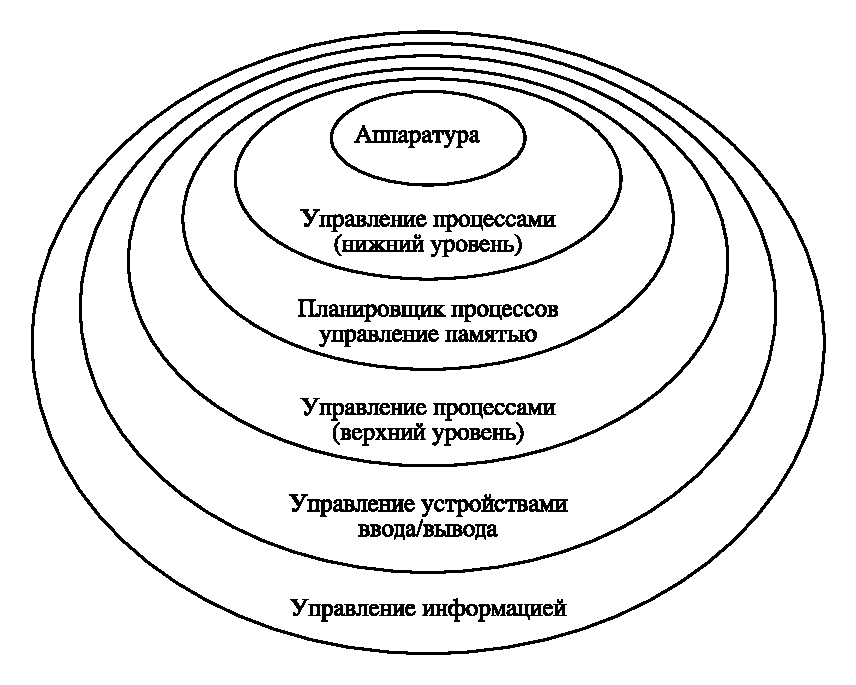
\includegraphics{os1}
\end{center}

Интерфейсы разделяются на:

\begin{itemize}
    \item Прозрачные - позволяет обращаться через уровни
    \item Полупрозрачные - какие то обращения доступны к вышележащему уровню
    \item Непрозрачные - строго к низлежащему уровню
\end{itemize}

\hfill

\hfill

\begin{table}[]
\caption{Структура ядра ОС UNIX 4.4 BSD}
\begin{tabular}{|c|c|c|c|c|c|c|c|c|}
\hline
\multicolumn{5}{|c|}{Системные вызовы} & //////////// & Сис. выз. & \multicolumn{2}{c|}{/////////////////} \\ \hline
\multicolumn{2}{|c|}{\begin{tabular}[c]{@{}c@{}}Управление\\ терминалом\end{tabular}} & 1 & 2 & 3 & 4 & Сокеты & \multirow{2}{*}{\begin{tabular}[c]{@{}c@{}}Обработка\\ сигналов\end{tabular}} & \multirow{2}{*}{\begin{tabular}[c]{@{}c@{}}Создание и\\ завершение\\ процесса\end{tabular}} \\ \cline{1-7}
\multirow{2}{*}{\begin{tabular}[c]{@{}c@{}}Необра-\\ ботан-\\ ный\\ телетайп\end{tabular}} & \begin{tabular}[c]{@{}c@{}}Обработанный\\ телетайп\end{tabular} & \multicolumn{2}{c|}{\begin{tabular}[c]{@{}c@{}}Файловая\\ система\end{tabular}} & \multicolumn{2}{c|}{\begin{tabular}[c]{@{}c@{}}Виртуальная\\ память\end{tabular}} & \begin{tabular}[c]{@{}c@{}}Сетевые\\ протоколы\end{tabular} &  &  \\ \cline{2-9}
 & \begin{tabular}[c]{@{}c@{}}Дисциплины\\ линий\\ связи\end{tabular} & \multicolumn{2}{c|}{\begin{tabular}[c]{@{}c@{}}Буферный\\ КЭШ\end{tabular}} & \multicolumn{2}{c|}{\begin{tabular}[c]{@{}c@{}}Страничный\\ КЭШ\end{tabular}} & \begin{tabular}[c]{@{}c@{}}Маршру-\\ тизация\end{tabular} & \multicolumn{2}{c|}{\begin{tabular}[c]{@{}c@{}}Планирование\\ процессов\end{tabular}} \\ \hline
\multicolumn{2}{|c|}{\begin{tabular}[c]{@{}c@{}}Драйверы символьных\\ устройств\end{tabular}} & \multicolumn{4}{c|}{\begin{tabular}[c]{@{}c@{}}Драйверы блочных\\ устройств\end{tabular}} & \begin{tabular}[c]{@{}c@{}}Сетевые\\ устрйства\end{tabular} & \multicolumn{2}{c|}{\begin{tabular}[c]{@{}c@{}}Диенетгеризация\\ процессов\end{tabular}} \\ \hline
\end{tabular}
\end{table}

\begin{enumerate}
    \item[1-] Символьный уровень
    \item[2-] Именование файлов
    \item[3-] Отображение адреса
    \item[4-] Страничные прерывания
    \item[///-] Аппаратные и эмулируемые прерывания
\end{enumerate}

\section{Управление процессорами}

Планирование и диспетчеризация процесса в процессе чего выделяется процессорное время.

\textbf{Планирование} (scheduling) - это постановка процесса в очередь на выполнение.

\textbf{Диспетчеризация} - непосредственно выделение процессу процессорного времени.

\subsection{Диаграмма состояния процесса}

Основная таблица - таблица процессов, она содержит дескрипторы (описатели)
процессов. Идентификатором процесса является номер строки в таблице процессов
(порядковый номер)

\begin{center}
    \includegraphics[scale=0.7]{os2}
\end{center}

В состоянии готовности находится большое количество процессов, которым необхоимо выделить процессорное время. Очередь выстраивается в соответствии с реализованний в системе дисциплиной планирования.

В состоянии завершения у программы забираются все ресурсы и созращаются в пулл свободных ресурсов

\subsection{Клонирование и диспетчеризация}

\paragraph{Классификация алгоритмов клонирования}

\textbf{Планировщик шедьюлер} (организация очереди процессов к какому либо ресурсу)

\begin{enumerate}
        \item С преключением (процесс может выполняться от начала и до конца) и без переключения (процесс может быть снят с управления)
        \item С приоритемами и без приоритетов
        \item С вытеснением (процесс может быть вытеснен другим процессом с более высоким приоритетом) и без вытеснения (вытеснение возможно только в системе с приоритетом)
\end{enumerate}

\paragraph{Мультипрограммная система пакетной обработки}

\begin{enumerate}
    \item \textbf{FIFO} - first in first out

        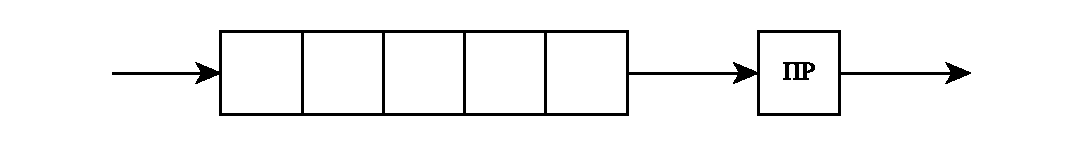
\includegraphics[scale=0.4]{os3}


    \item \textbf{SJF} - shortest job first. Приводило к бесконечному откладыванию, то есть задания с большим процессорным временем все время откладывались в конец очереди

    \item \textbf{SRT} - shortest reaming time (наименьшее оставшееся время). Процесс может быть прерван если поступит процесс с меньшим оценочным временем выполнения, чем время оставшееся текущему процессу до его завершения (на основе заявленного времени). Усугубляет ситацию с бесконечным откладыванием.

    \item HRN - highest response rationext (наибольшее относительное время ответа). Приоритет вычисляется по формуле

        $$
        \frac{t_w + t_s}{t_s}, \text{ где } t_w \text{ - время ожидания}, t_s \text{ - запрошенное время}
        $$

\end{enumerate}

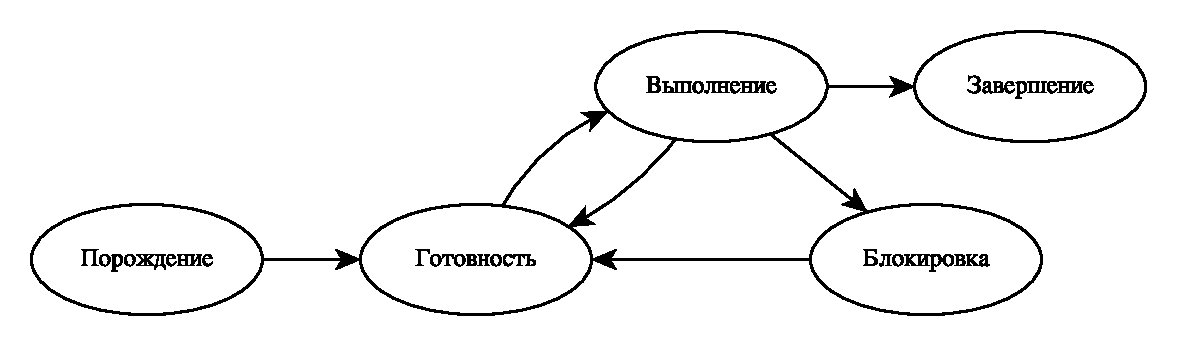
\includegraphics[scale=0.7]{os4}

\subsection{Планирование в системах разделения времени}

Время в системах выдается квантами.

\begin{enumerate}
    \item RR - циклическое планирование, процессы выстраиваются в очередь, но по истечении кванта ставятся в конец очереди

        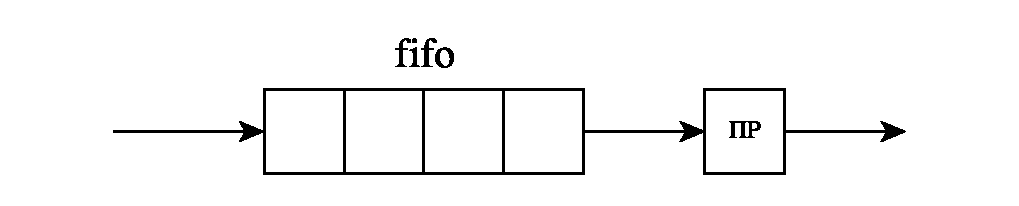
\includegraphics[scale=0.4]{os5}

    \item Многоуровневые очереди или алгоритм адаптивного планирования

        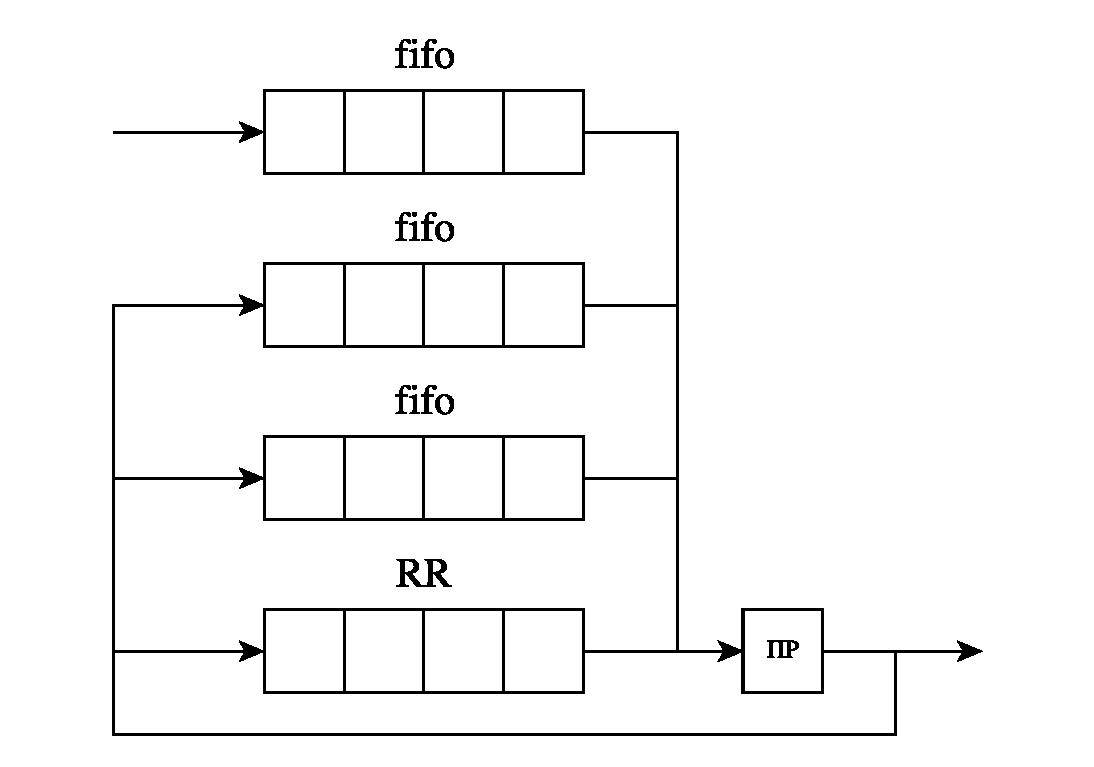
\includegraphics[scale=0.4]{os6}

        В первую очередь с наивысшим приоритетом поступают только что созданные процессы или завершившие блокировку в ожидании завершения ввода-вывода. Для 1 очереди квант процесса выбирается таким образом, чтобы наибольшее число процессов успело или завершится или выдаст запрос на ввод-вывод. Если процесс не успел завершится за по истечении кванта он поступает в слудющую очередь с более низким приоритетом, и так далее пока не окажется в пследней очереди с самым низким приоритетом по алгоритму. В этой очереди крутится так называемый "холостой процесс", поскольку система не может ничего не делать.

        Пересчитываться могут только пользовательские приоритеты (приложений). Старается быть справедливым, чтобы у всех процессов было примерно одинаковое время, но также учитывается время простоя процесса. В старом UNIX используется формула.
\end{enumerate}

Интерактивные - процессы, запрашивающие ввод-вывод с клавиатуры, мыши. Самые высокоприоритетные операции.

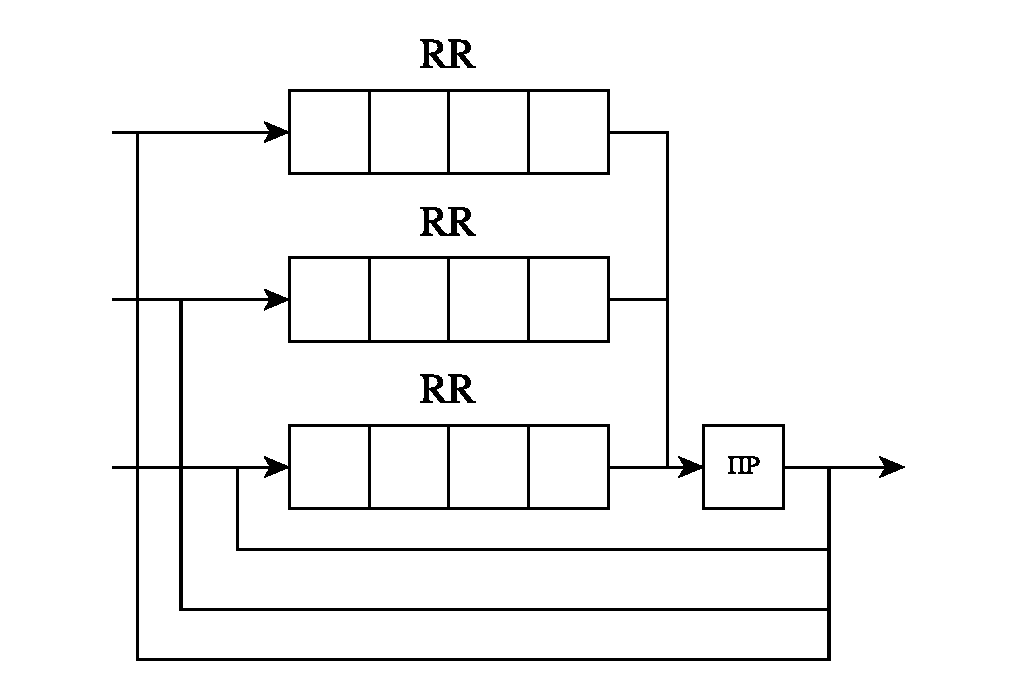
\includegraphics[scale=0.4]{os7}

\subsection{Уровни наблюдения}

\begin{enumerate}
    \item Последоетельное выполнение
    \item Квант выполняется 1 процесс, квант - другой (квазипараллельное). С точки зрения пользователя программы выполняются параллельно, с точки зрения процесса - последовательно
    \item Параллельное выполнение. Реально параллельное, по времени совмещается выполение команд программы.
\end{enumerate}

Выполнение $\to$ готовность - вытеснен или истек квант

Выполнение $\to$ блокировка - запрос дополнительного ресурса

\section{Переключение в режим ядра}

Процесс - главная абстракция системы. UNIX декларирует следующим образом: процесс часть времени выполняет собственный код, и тогда он выполняется в \textbf{режиме задачи}, а часть времени выполняет реинтерабельный код операционной системы, и тогда он выпоняется в \textbf{режиме ядра}.

Системные вызовы - запрос процесса на системные ресурсы (ввод-вывод). Ни одна операционная система не позволяет процессу напрямую обратиться к устройствам к устройствам ввода-вывода. Если бы обращались напрямую, то такая система была бы незащищенной. Для обслуживания системного вызова процесс должен перейти в режим ядра, в режиме ядра выполняется реентерабельный код операционной системы. Реентерабельный код - код чистой процедуры (чистая процедура не содифицирует саму себя, то есть вынесены все данные). Коды ядра работают с системными таблицами (коды ядра реентерабельны). Процедуры сами являются ресурсами, которые могут запрашивать процессы, разные процессы могут находится в разных точках одной и той же процедуры. При выполнении системнго вызова процесс переключается в режим ядра и выполняет реентерабельный код операционной системы. После того, как итемный вызов обслужен, процесс опять переключается в режим задачи и выполняет собственный код.

В режиме ядра процесс переносится в очередь готовых процессов, выполняют действия для конкретного процесса. Затем когда процесс получает квант, он начинает выполнять собственный код. Если процесс запросил дополнитеьный ресурс, то процесс переключится в режим ядра и будет блокирован, будет находится в режиме блокировки пока процесс не получит нужный ему ресурс, после чего система поместит процесс в очередь готовых процессов и после получения кванта процесс может продолжить выполнение своего кода до конца.

Три события, переводящих систему в режим ядра

\begin{enumerate}
    \item Системные вызовы
    \item Исключения
    \item Аппаратные прерывания
\end{enumerate}

\section{Переключение контекста}

\textbf{Аппратный контекст} - регистры процессора (не все)

Сохранение регистров поддерживается аппаратно.

Полный контекст состоит из аппаратного контекста и информации о выделенных процессу ресурсах, в частности о выделенной процессу памяти. Это структуры. Все в системе описывается соответствующими структурами.

UNIX BSD $\to$ struct proc

UNIX $\to$ struct task\_struct

Вся эта информация нужна системе для того, чтобы иметь возможность выполнения процесса. Понятие контекста является важнейшим в системе.

Полный контекст переклчючается тогда, когда процесс возвращается в готовность или ...

Диаграмма состояний процесса в UNIX

Любой процесс вызывается системным вызовом Fork. Он создает новый процесс.

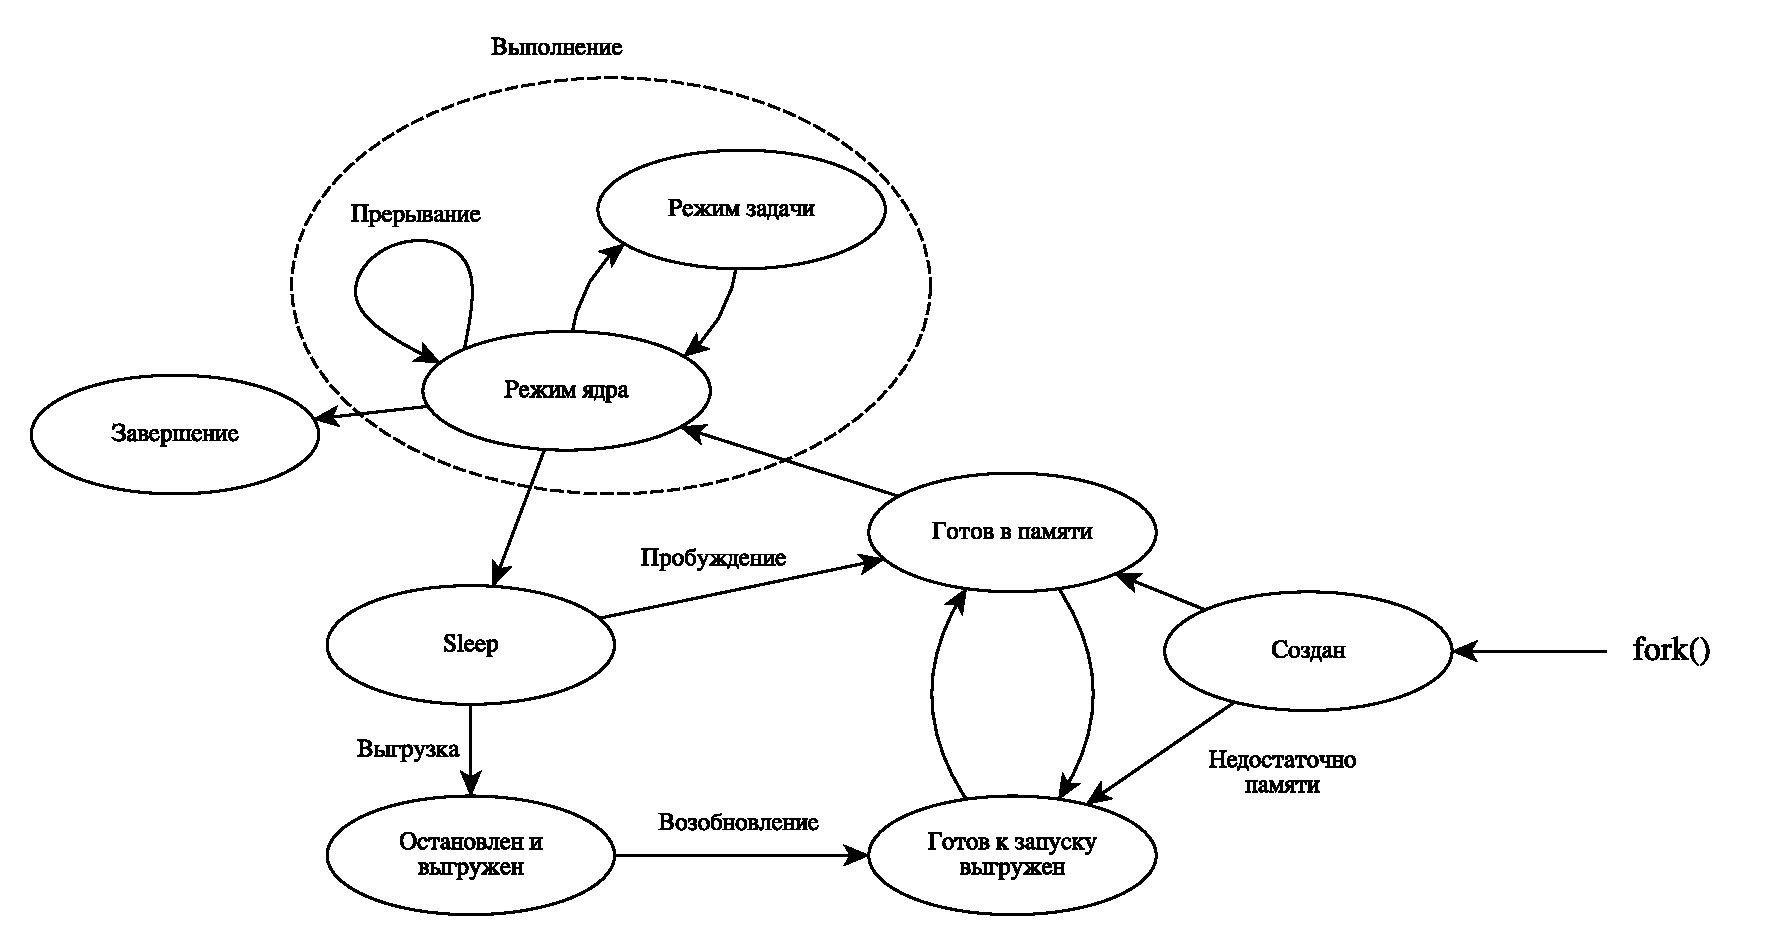
\includegraphics[scale=0.5]{os8}

\section{Потоки}

Чтобы сократить накладные расходы на переключение контекста (это очень затратно)

Возникло два типа потоков

\begin{enumerate}
    \item Потоки на уровне пользователя
    \item Потоки на уровне ядра
\end{enumerate}

В качестве потока выделяются части кода процесса, которые могут выполняться параллельно с другими частями кода процессора. В любом случае владельцем ресурсов в процессе является процесс. Поток выполняется в адресном пространстве процесса (так как не имеет своего адресного пространства). Поток оказывается владельцем счетчика команд (аппаратного контекста).

Существут многопоточные и однопоточные модели процесса.

\subsection{Однопоточная модель}

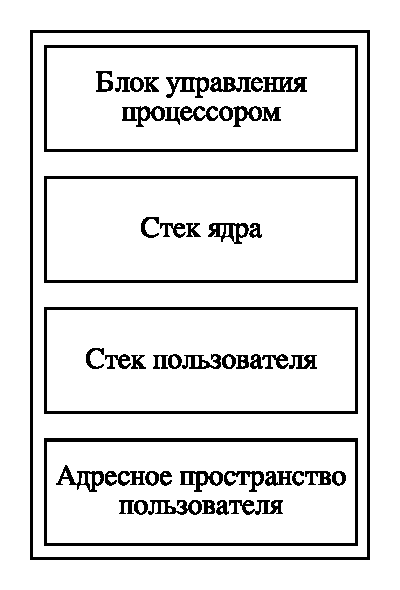
\includegraphics{os9}

\end{document}
